\documentclass[a4paper,12pt]{article}
\usepackage[top = 2.5cm, bottom = 2.5cm, left = 2.5cm, right = 2.5cm]{geometry}
\usepackage[T1]{fontenc}
\usepackage[utf8]{inputenc}
\usepackage{multirow} 
\usepackage{booktabs} 
\usepackage{graphicx}
\usepackage[spanish]{babel}
\usepackage{setspace}
\setlength{\parindent}{0in}
\usepackage{float}
\usepackage{fancyhdr}
\usepackage{amsmath}
\usepackage{amssymb}
\usepackage{amsthm}
\usepackage[numbers]{natbib}
\newcommand\Mycite[1]{%
	\citeauthor{#1}~[\citeyear{#1}]}
\usepackage{graphicx}
\usepackage{subcaption}
\usepackage{booktabs}
\usepackage{etoolbox}
\usepackage{minibox}
\usepackage{hyperref}
\usepackage{xcolor}
\usepackage[normalem]{ulem}
 \useunder{\uline}{\ul}{}
\usepackage[skins]{tcolorbox}
%---------------------------

\newtcolorbox{cajita}[1][]{
	 #1
}

\newenvironment{sol}
{\renewcommand\qedsymbol{$\square$}\begin{proof}[\textbf{Solución.}]}
	{\end{proof}}

\newenvironment{dem}
{\renewcommand\qedsymbol{$\blacksquare$}\begin{proof}[\textbf{Demostración.}]}
	{\end{proof}}

\newtheorem{problema}{Problema}
\newtheorem{definicion}{Definición}
\newtheorem{ejemplo}{Ejemplo}
\newtheorem{teorema}{Teorema}
\newtheorem{corolario}{Corolario}[teorema]
\newtheorem{lema}[teorema]{Lema}
\newtheorem{prop}{Proposición}
\newtheorem*{nota}{\textbf{NOTA}}
\renewcommand\qedsymbol{$\blacksquare$}
\usepackage{svg}
\usepackage{tikz}
\usepackage[framemethod=default]{mdframed}
\global\mdfdefinestyle{exampledefault}{%
linecolor=lightgray,linewidth=1pt,%
leftmargin=1cm,rightmargin=1cm,
}




\newenvironment{noter}[1]{%
\mdfsetup{%
frametitle={\tikz\node[fill=white,rectangle,inner sep=0pt,outer sep=0pt]{#1};},
frametitleaboveskip=-0.5\ht\strutbox,
frametitlealignment=\raggedright
}%
\begin{mdframed}[style=exampledefault]
}{\end{mdframed}}
\newcommand{\linea}{\noindent\rule{\textwidth}{3pt}}
\newcommand{\linita}{\noindent\rule{\textwidth}{1pt}}

\AtBeginEnvironment{align}{\setcounter{equation}{0}}
\pagestyle{fancy}

\fancyhf{}









%----------------------------------------------------------
\lhead{\footnotesize Geometría Moderna}
\rhead{\footnotesize  Rudik Roberto Rompich}
\cfoot{\footnotesize \thepage}


%--------------------------

\begin{document}
 \thispagestyle{empty} 
    \begin{tabular}{p{15.5cm}}
    \begin{tabbing}
    \textbf{Universidad del Valle de Guatemala} \\
    Departamento de Matemática\\
    Licenciatura en Matemática Aplicada\\\\
   \textbf{Estudiante:} Rudik Roberto Rompich\\
   \textbf{Correo:}  \href{mailto:rom19857@uvg.edu.gt}{rom19857@uvg.edu.gt}\\
   \textbf{Carné:} 19857
    \end{tabbing}
    \begin{center}
        MM2031 - Geometría Moderna - Catedrático: María Eugenia Contreras Pinillos\\
        \today
    \end{center}\\
    \hline
    \\
    \end{tabular} 
    \vspace*{0.3cm} 
    \begin{center} 
    {\Large \bf  HT 1
} 
        \vspace{2mm}
    \end{center}
    \vspace{0.4cm}
%--------------------------

\section{Problema 1}
\begin{enumerate}
	\item Localice en un plano los puntos $A(1,1)$, $B(3,4)$, $C(-2,5)$ y $D(-3,2)$. 
	\item Una de los puntos para obtener el cuadrilátero $ABCD$. 
	\item Aplique ahora las siguientes transformaciones al cuadrilátero original: 
	\begin{enumerate}
		\item Una traslación en dirección del vector $0A$. 
		\item Reflexión respecto al punto $E(-2,2)$. 
		\item Homotecia respecto al origen $(0,0)$ de $k=-(0.5)$. 
	\end{enumerate}
\end{enumerate}



\begin{problema}
	Dado un cuadrado determinar las transformaciones que llevan al cuadrado sobre el mismo. Luego completar la tabla con la composición de transformaciones como lo hicimos con el triángulo equilátero.
\end{problema}

\begin{sol}
	Se propone encontrar los ejes de simetría del cuadrado por medio de sus bisectrices y mediatrices, tal que 
	
		\begin{figure}[H]
		\centering
		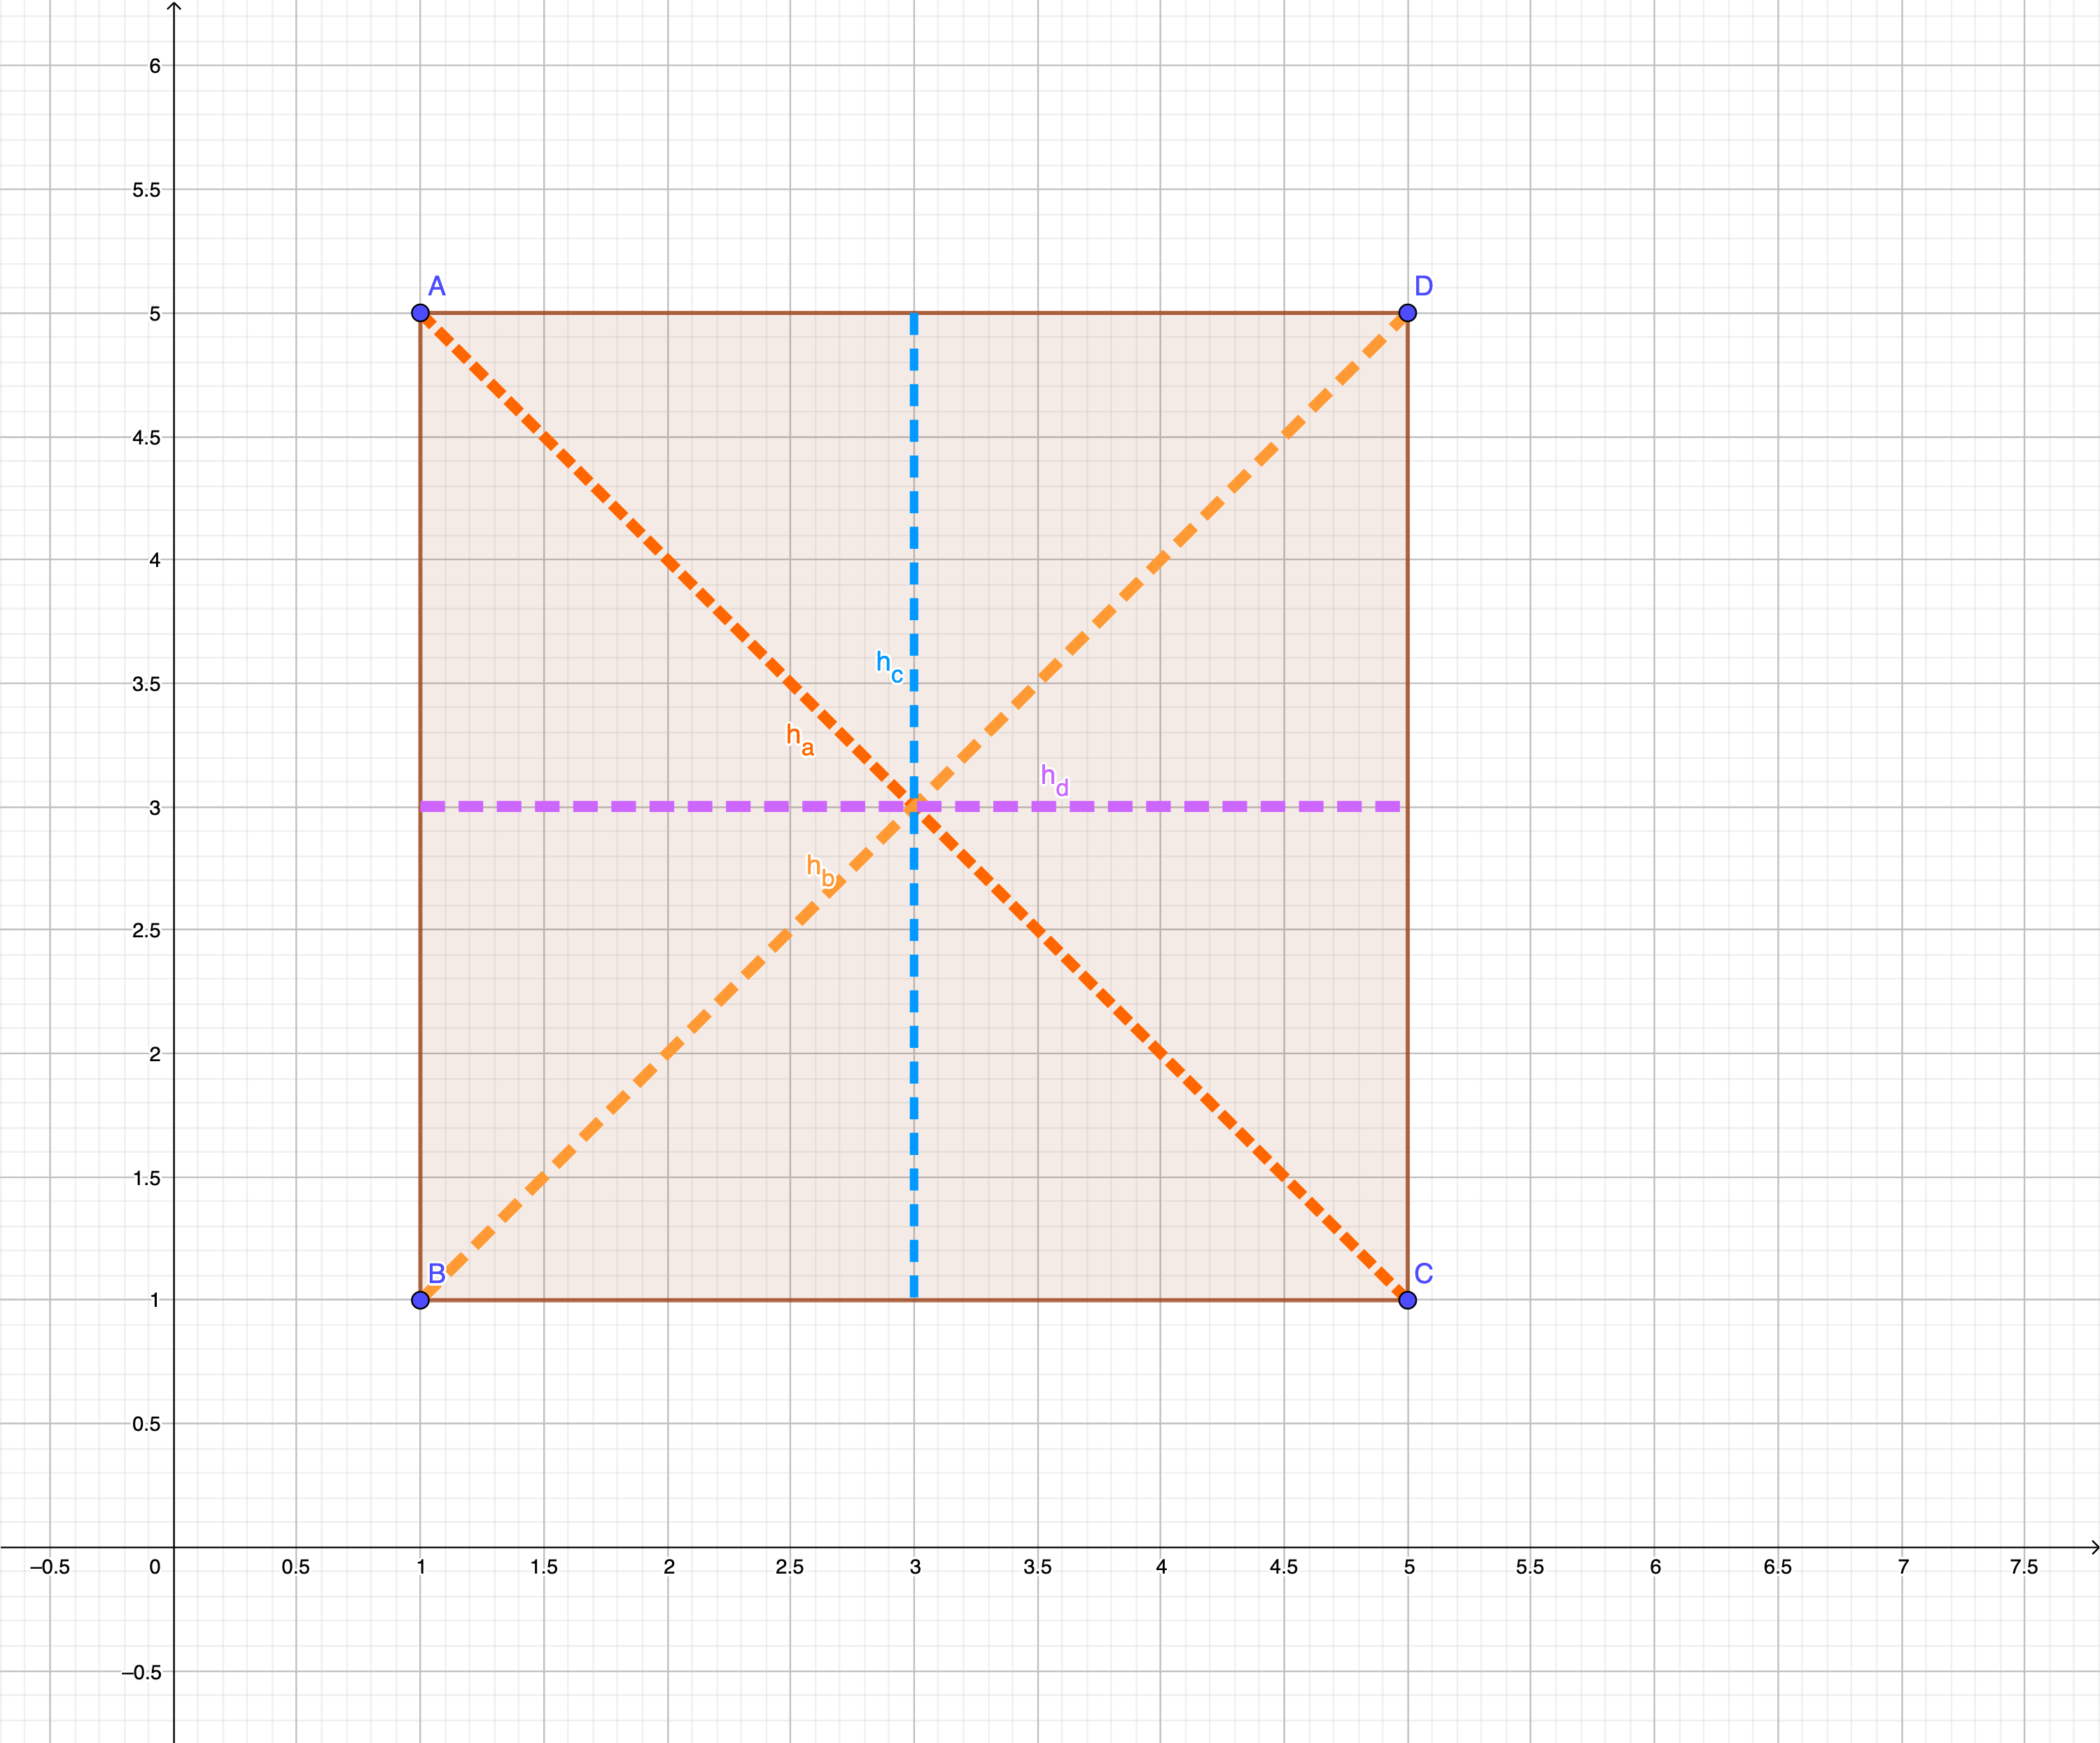
\includegraphics[scale=1.5]{Images/P2-1.png}
	\end{figure}

Entonces, una de sus transformaciones que llevan al cuadrado sobre el mismo es: 

$$\operatorname{Rot}(H, 360^{\circ}).$$

Nombraremos el cuadrado como: $\square ABCD$, procedemos a hacer el cuadro: 

% Please add the following required packages to your document preamble:
% \usepackage[normalem]{ulem}
% \useunder{\uline}{\ul}{}
\begin{table}[H]
	\centering 
	\begin{tabular}{|c|c|c|c|c|c|c|c|c|}
		\hline
		\textit{\textbf{0}}      & {\ul \textit{$R_{0}$}}      & {\ul \textit{$R_{90}$}}     & {\ul \textit{$R_{180}$}}    & {\ul \textit{$R_{270}$}}    & {\ul \textit{$h_d$}}        & {\ul \textit{$h_c$}}        & {\ul \textit{$h_a$}}        & {\ul \textit{$h_b$}}        \\ \hline
		{\ul \textit{$R_{0}$}}   & \textit{\textbf{$R_{0}$}}   & \textit{\textbf{$R_{90}$}}  & \textit{\textbf{$R_{180}$}} & \textit{\textbf{$R_{270}$}} & \textit{\textbf{$h_d$}}     & \textit{\textbf{$h_c$}}     & \textit{\textbf{$h_a$}}     & \textit{\textbf{$h_b$}}     \\ \hline
		{\ul \textit{$R_{90}$}}  & \textit{\textbf{$R_{90}$}}  & \textit{\textbf{$R_{180}$}} & \textit{\textbf{$R_{270}$}} & \textit{\textbf{$R_{0}$}}   & \textit{\textbf{$h_b$}}     & \textit{\textbf{$h_a$}}     & \textit{\textbf{$h_d$}}     & \textit{\textbf{$h_c$}}     \\ \hline
		{\ul \textit{$R_{180}$}} & \textit{\textbf{$R_{180}$}} & \textit{\textbf{$R_{270}$}} & \textit{\textbf{$R_{0}$}}   & \textit{\textbf{$R_{90}$}}  & \textit{\textbf{$h_c$}}     & \textit{\textbf{$h_d$}}     & \textit{\textbf{$h_b$}}     & \textit{\textbf{$h_a$}}     \\ \hline
		{\ul \textit{$R_{270}$}} & \textit{\textbf{$R_{270}$}} & \textit{\textbf{$R_{0}$}}   & \textit{\textbf{$R_{90}$}}  & \textit{\textbf{$R_{180}$}} & \textit{\textbf{$h_a$}}     & \textit{\textbf{$h_b$}}     & \textit{\textbf{$h_c$}}     & \textit{\textbf{$h_d$}}     \\ \hline
		{\ul \textit{$h_d$}}     & \textit{\textbf{$h_d$}}     & \textit{\textbf{$h_a$}}     & \textit{\textbf{$h_c$}}     & \textit{\textbf{$h_b$}}     & \textit{\textbf{$R_0$}}     & \textit{\textbf{$R_{180}$}} & \textit{\textbf{$R_{90}$}}  & \textit{\textbf{$R_{270}$}} \\ \hline
		{\ul \textit{$h_c$}}     & \textit{\textbf{$h_c$}}     & \textit{\textbf{$h_b$}}     & \textit{\textbf{$h_d$}}     & \textit{\textbf{$h_a$}}     & \textit{\textbf{$R_{180}$}} & \textit{\textbf{$R_0$}}     & \textit{\textbf{$R_{270}$}} & \textit{\textbf{$R_{90}$}}  \\ \hline
		{\ul \textit{$h_a$}}     & \textit{\textbf{$h_a$}}     & \textit{\textbf{$h_c$}}     & \textit{\textbf{$h_b$}}     & \textit{\textbf{$h_d$}}     & \textit{\textbf{$R_{270}$}} & \textit{\textbf{$R_{90}$}}  & \textit{\textbf{$R_0$}}     & \textit{\textbf{$R_{180}$}} \\ \hline
		{\ul \textit{$h_b$}}     & \textit{\textbf{$h_b$}}     & \textit{\textbf{$h_d$}}     & \textit{\textbf{$h_a$}}     & \textit{\textbf{$h_c$}}     & \textit{\textbf{$R_{90}$}}  & \textit{\textbf{$R_{270}$}} & \textit{\textbf{$R_{180}$}} & \textit{\textbf{$R_0$}}     \\ \hline
	\end{tabular}
\end{table}
\end{sol}

\begin{problema}
	Dado el poligono cuyos vértices se encuentran en los puntos:
	$$
	A=(3,3), B=(5,1), \quad C=(7,1), \quad D=(9,3), E=(9,5)
	$$
	Aplique las siguientes transformaciones: 
	\begin{enumerate}
		\item Rotación $=\operatorname{rot}\left(\mathrm{D}, 90^{\circ}\right)$
		\item Reflexión: $\operatorname{Ref} \overrightarrow{A E}$
	    \item Traslación $=\operatorname{Tra}(\overrightarrow{A C})$
	    \item Homotecia $=\operatorname{Hom}\left(O(0,0), k=\frac{1}{2}\right)$
	\end{enumerate}

	En el siguiente orden:
	
	$$
	\operatorname{rot}\left(D, 90^{\circ}\right) \circ \operatorname{Ref} \overrightarrow{A E} \circ \operatorname{Tra}(\overrightarrow{A C}) \circ \operatorname{Hom}\left(\mathrm{O}(0,0), \mathrm{k}=\frac{1}{2}\right)
	$$
\end{problema}

\begin{sol}
	Aplicando las siguientes transformaciones: 
		\begin{enumerate}
		\item Rotación $=\operatorname{rot}\left(\mathrm{D}, 90^{\circ}\right)$ - \textcolor{blue}{Celeste}
		\item Reflexión: $\operatorname{Ref} \overrightarrow{A E}$ - \textcolor{orange}{Naranja}
		\item Traslación $=\operatorname{Tra}(\overrightarrow{A C})$- \textcolor{green}{Verde}
		\item Homotecia $=\operatorname{Hom}\left(O(0,0), k=\frac{1}{2}\right)$ - \textcolor{purple}{Morado}
	\end{enumerate}

Comenzamos con la \textbf{homotecia}: 

$$\begin{cases}
	H(x,y)= (\frac{1}{2}x,\frac{1}{2}y)\\
	A'(3,3)= (3/2,3/2)\\
	B'(5,1)= (5/2,1/2)\\
	C'(7,1)= (7/2,1/2)\\
	D'(9,3)= (9/2,3/2)\\
	E'(9,5)=(9/2,5/2)
\end{cases}$$
\textbf{Traslación}, definida como $\operatorname{Tra}\overrightarrow{AC}= (7-3,1-3)=(4,-2)$

$$\begin{cases}
	\operatorname{Tra}(x'',y'')= (x''+4,y''-2)\\
	A''(3/2,3/2)= (11/2,-1/2)\\
	B''(5/2,1/2)= (13/2,-3/2)\\
	C''(7/2,1/2)= (15/2,-3/2)\\
	D''(9/2,3/2)= (17/2,-1/2)\\
	E''(9/2,5/2)=(17/2,1/2)
\end{cases}$$

\textbf{Reflexión}, la reflexión sobre la recta se obtiene con el $(p, q)$ respecto a la recta  $ay + bx + c = 0$ definido como

$$\left(\frac{p(a^{2}-b^{2})-2b(aq+c)}{a^{2}+b^{2}},\frac{q(b^{2}-a^{2})-2a(bp+c)}{a^{2}+b^{2}}\right)$$
Finalmente, la \textbf{rotación}, se obtiene con (ángulos en radianes): 

$$X = B_X + (A_X-B_X)\cos\phi  - (A_Y-B_Y)\sin \phi $$
$$Y = B_Y + (A_X-B_X)\sin\phi  + (A_Y-B_Y)\cos \phi $$
	\begin{figure}[H]
		\centering
		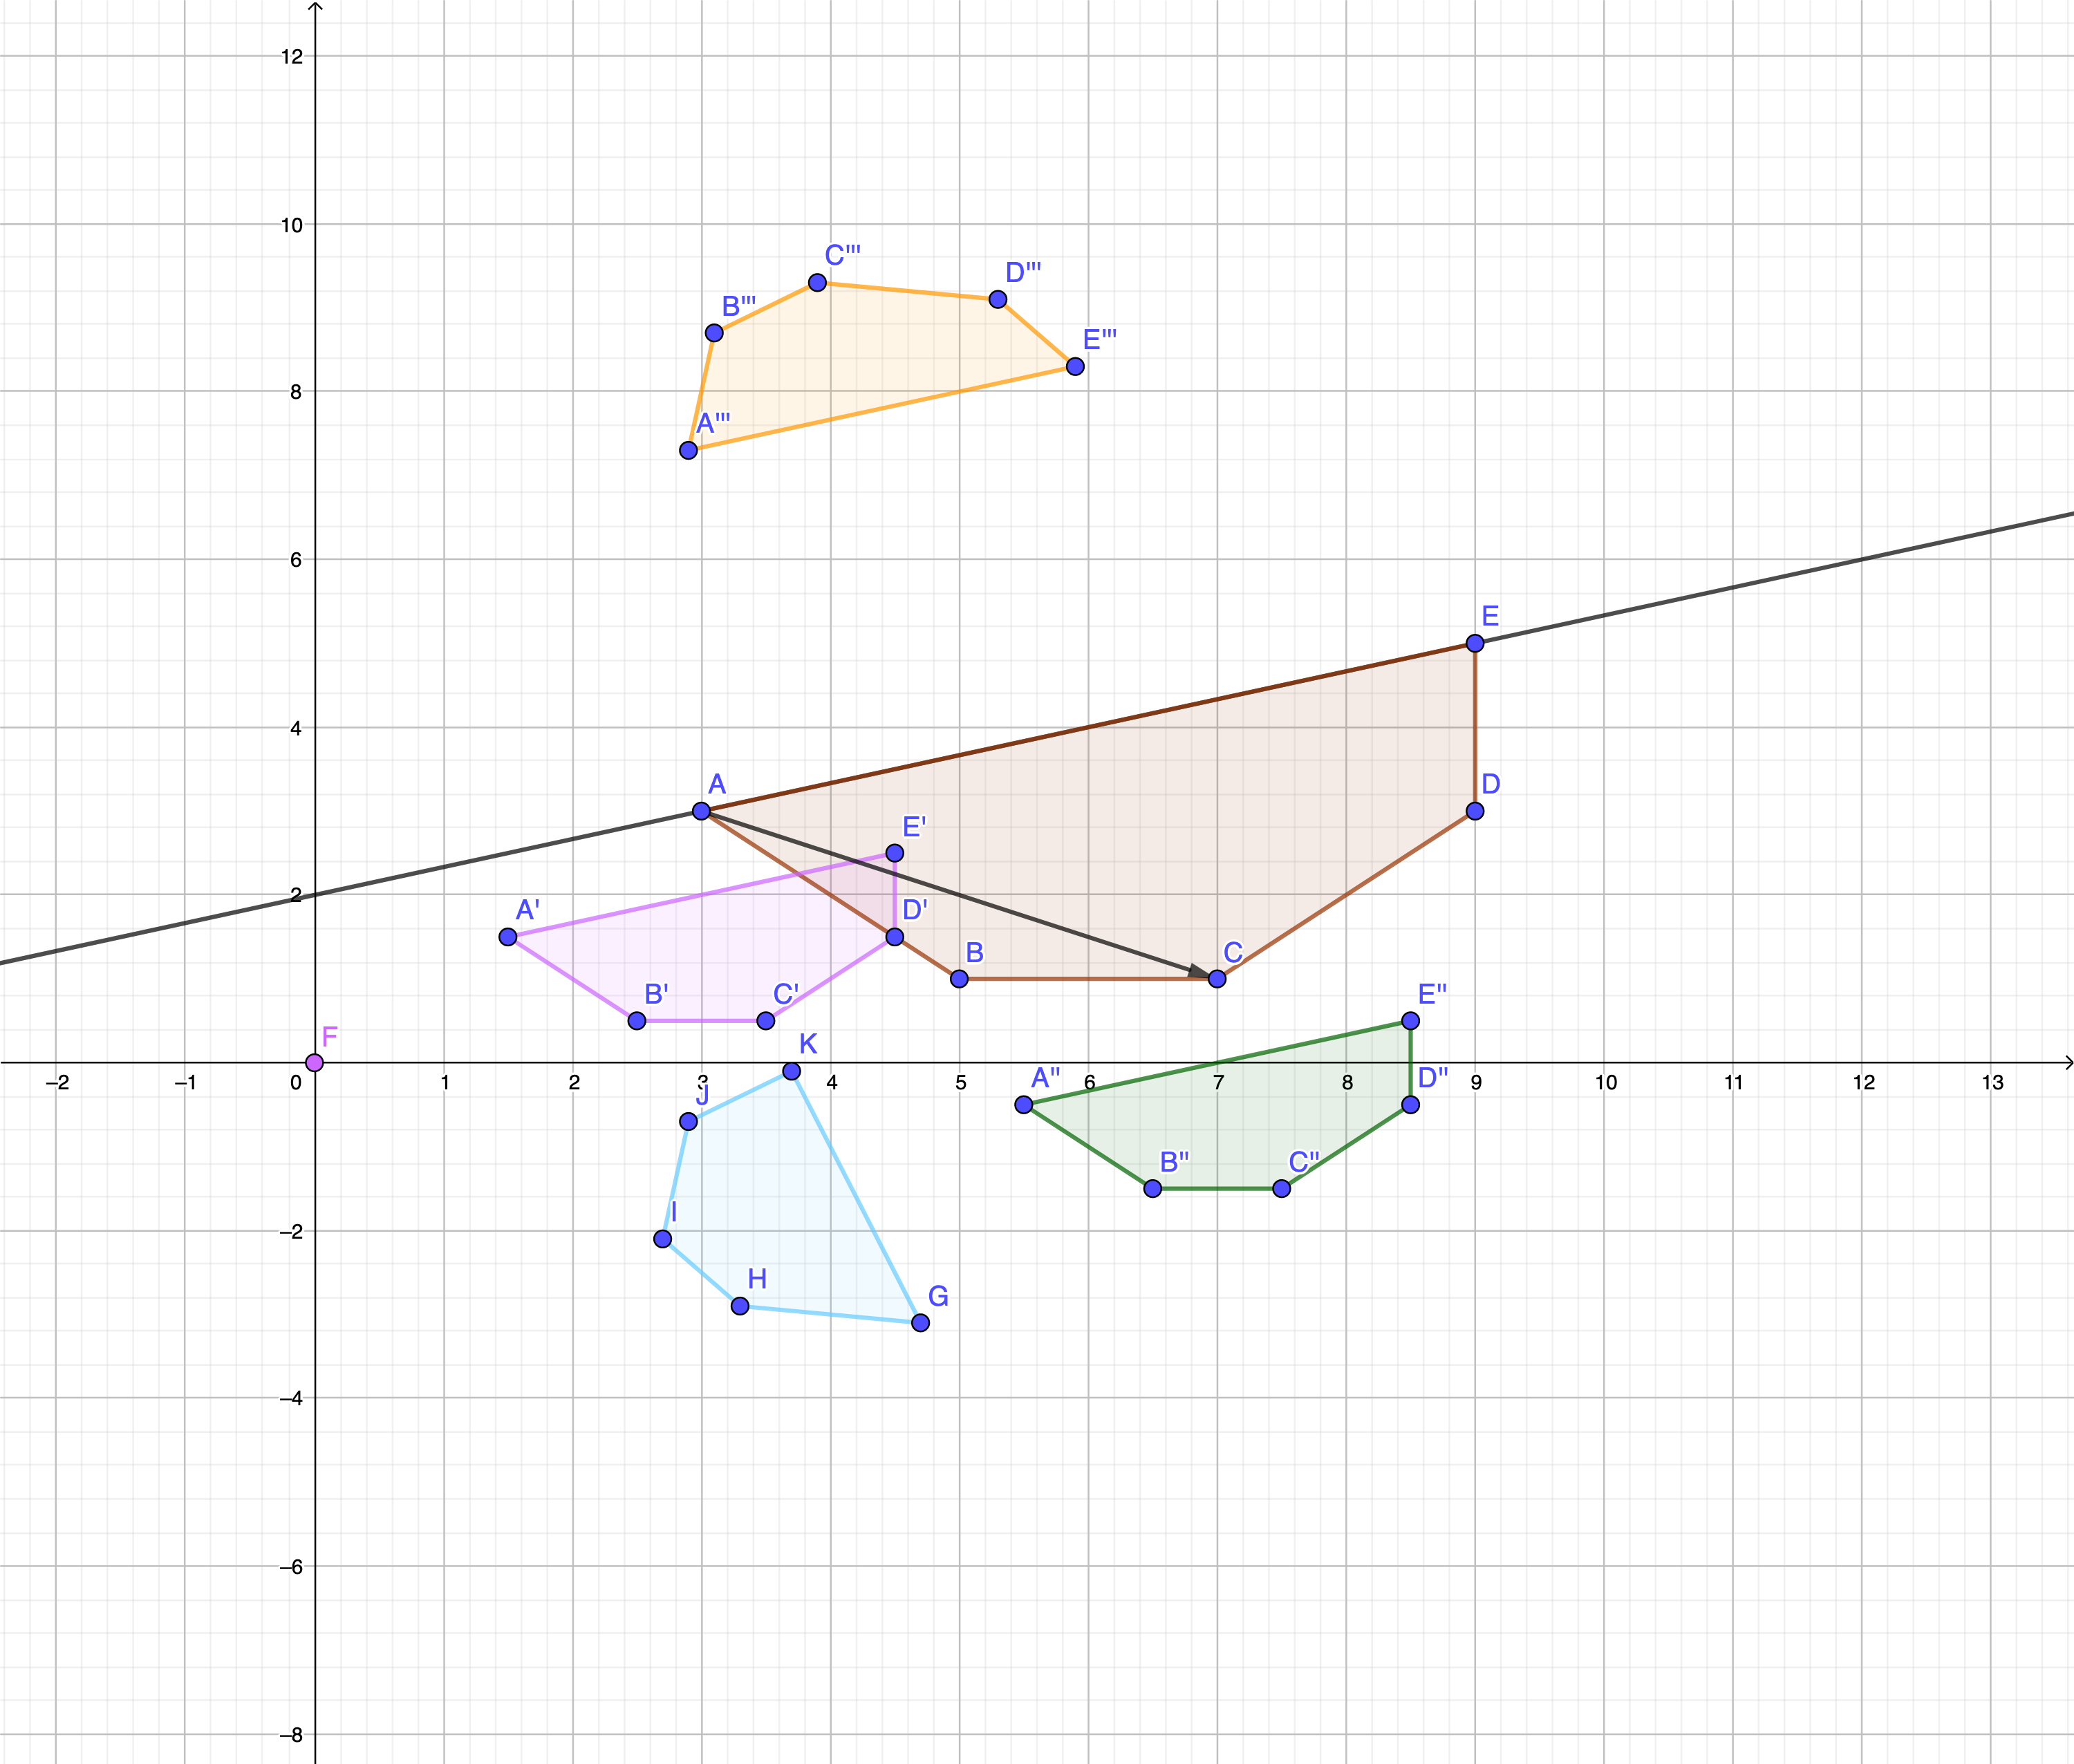
\includegraphics[scale=1]{Images/P3-1.png}
	\end{figure}

\end{sol}
\begin{problema}
	Si A,B y C son puntos colineales distintos, P,Q y R son los puntos medios de $\mathrm{BC}, \mathrm{CA}$ y $\mathrm{AB}$ respectivamente muestre que el punto medio de CR coincide con el punto medio de PQ (Haga una construcción)
\end{problema}
	\begin{figure}[H]
	\centering
	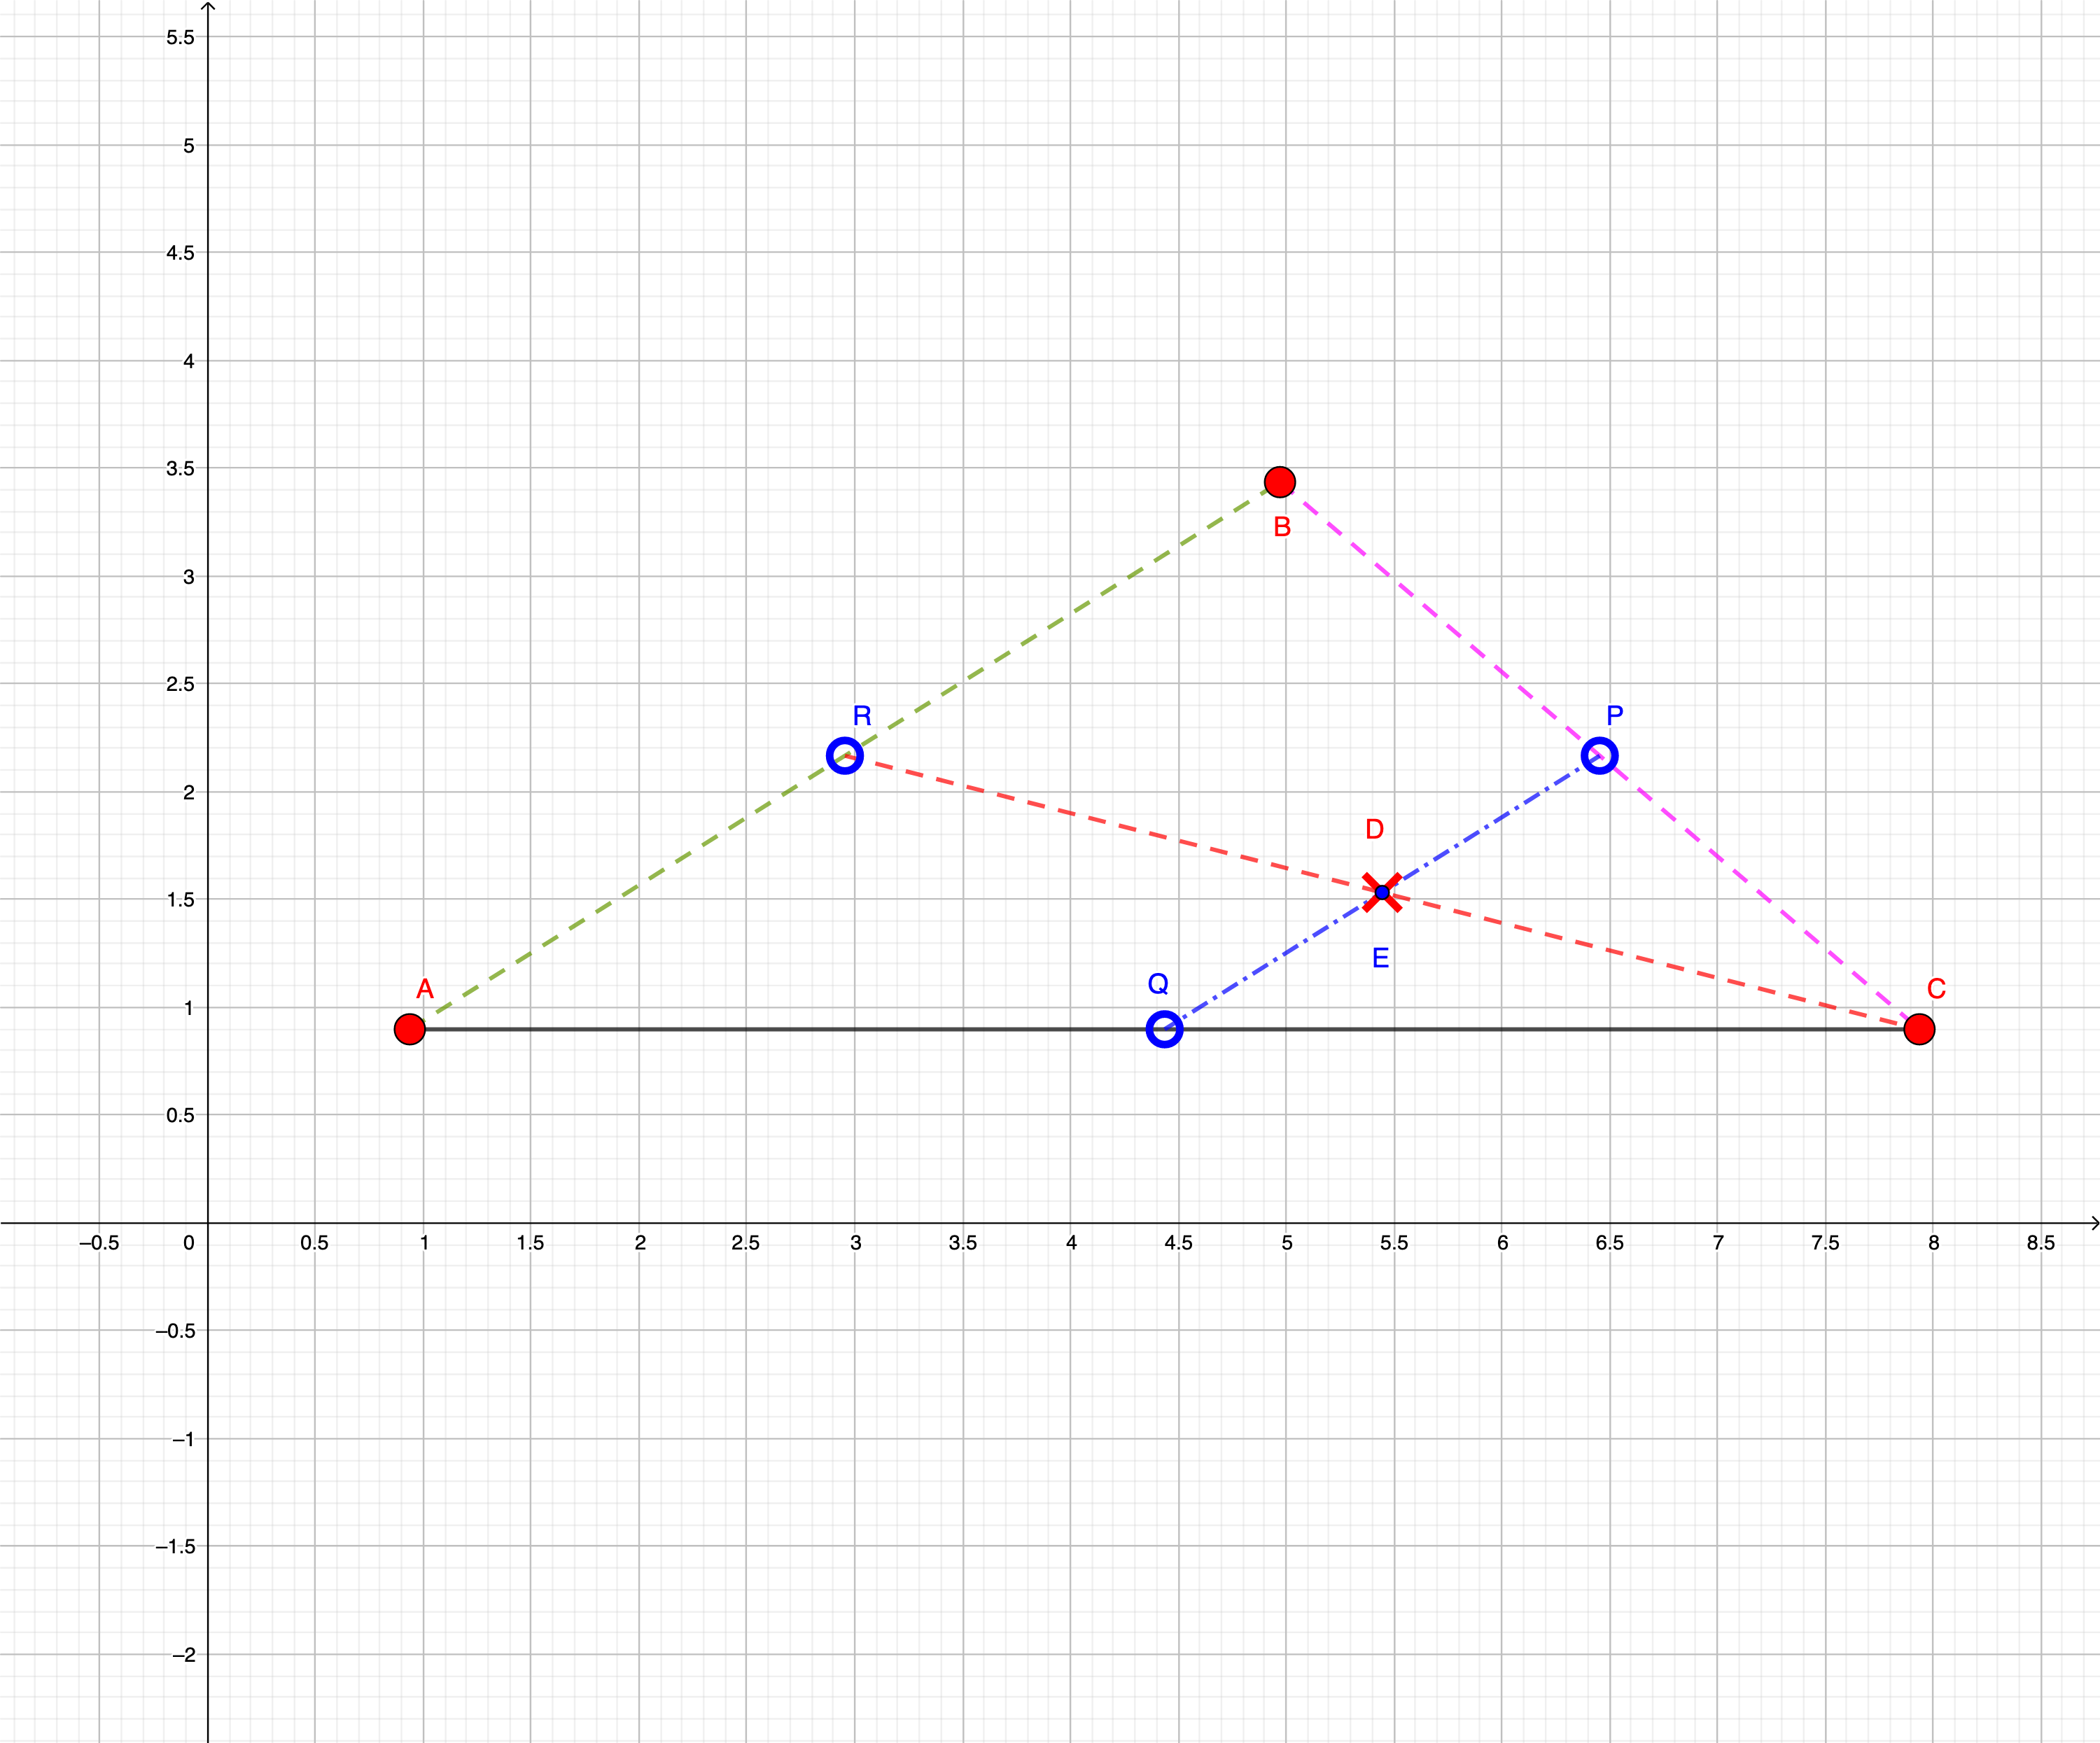
\includegraphics[scale=1]{Images/P4.png}
	\caption{Construcción}
\end{figure}
	\begin{figure}[H]
	\centering
	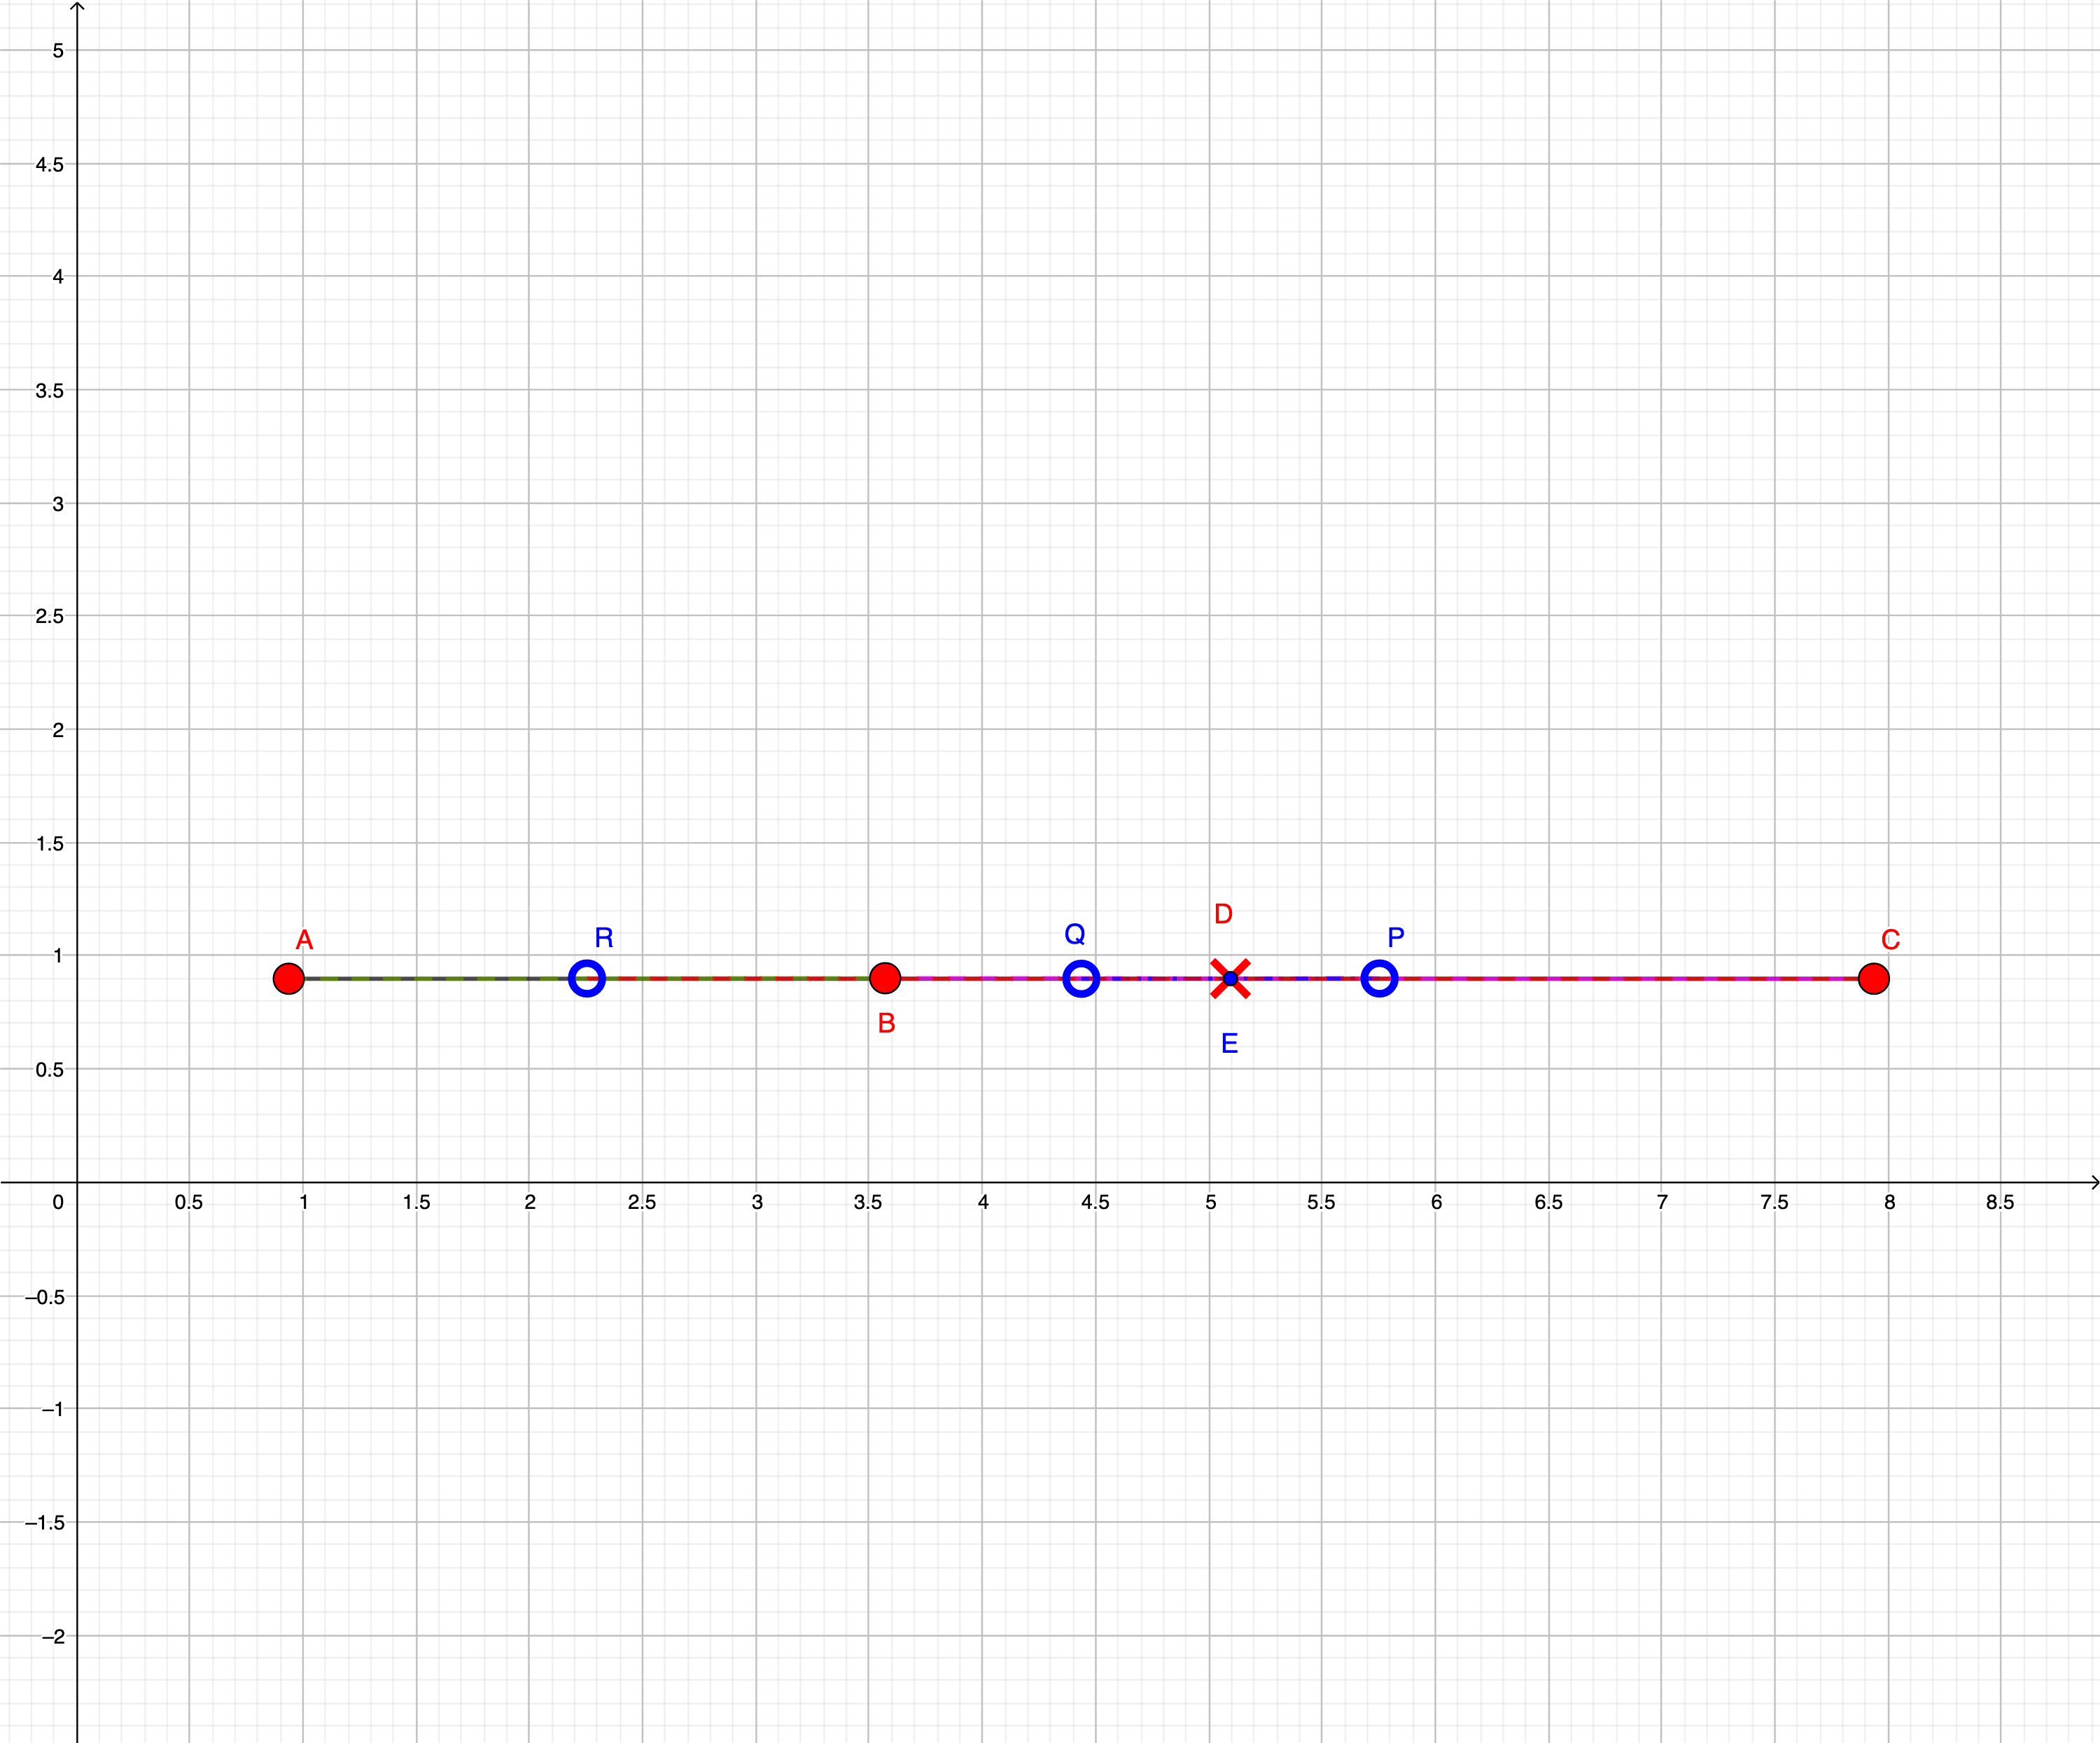
\includegraphics[scale=1]{Images/P4-1.png}
	\caption{Construcción}
\end{figure}

\begin{proof}
	Vamos a considerar la definición de punto medio como: 
	$$M=\frac{1}{2}(A+B).$$
	Por hipótesis, tenemos 3 puntos medio definidos como:
	$$P=\frac{1}{2}(B+C), Q=\frac{1}{2}(C+A), R=\frac{1}{2}(A+B).$$
	
	Ahora bien, nos piden mostrar que 
	$$D=\frac{1}{2}(C+R), E=\frac{1}{2}(P+Q) \ni D=E.$$
	
	Por lo que procedemos a calcular $D$ y $E$: 
	\begin{itemize}
		\item $D=\frac{1}{2}(C+R)=\frac{1}{2}\left[C+\frac{1}{2}\left(A+B\right)\right]=\frac{1}{4}A+\frac{1}{4}B+\frac{1}{2}C.$
		\item $ E=\frac{1}{2}(P+Q) = \frac{1}{2}\left[\frac{1}{2}(B+C)+\frac{1}{2}(A+C)\right]=\frac{1}{4}A+\frac{1}{4}B+\frac{1}{2}C$
	\end{itemize}
$$\therefore \ D=E.$$
\end{proof}

\begin{problema}
	Muestre que si $P$ es el punto medio de $B C$ en el triángulo $A B C, y$ si $A B$ es menor que AC entonces el ángulo PAC es menor que el ángulo BAP.
\end{problema}

	\begin{figure}[H]
	\centering
	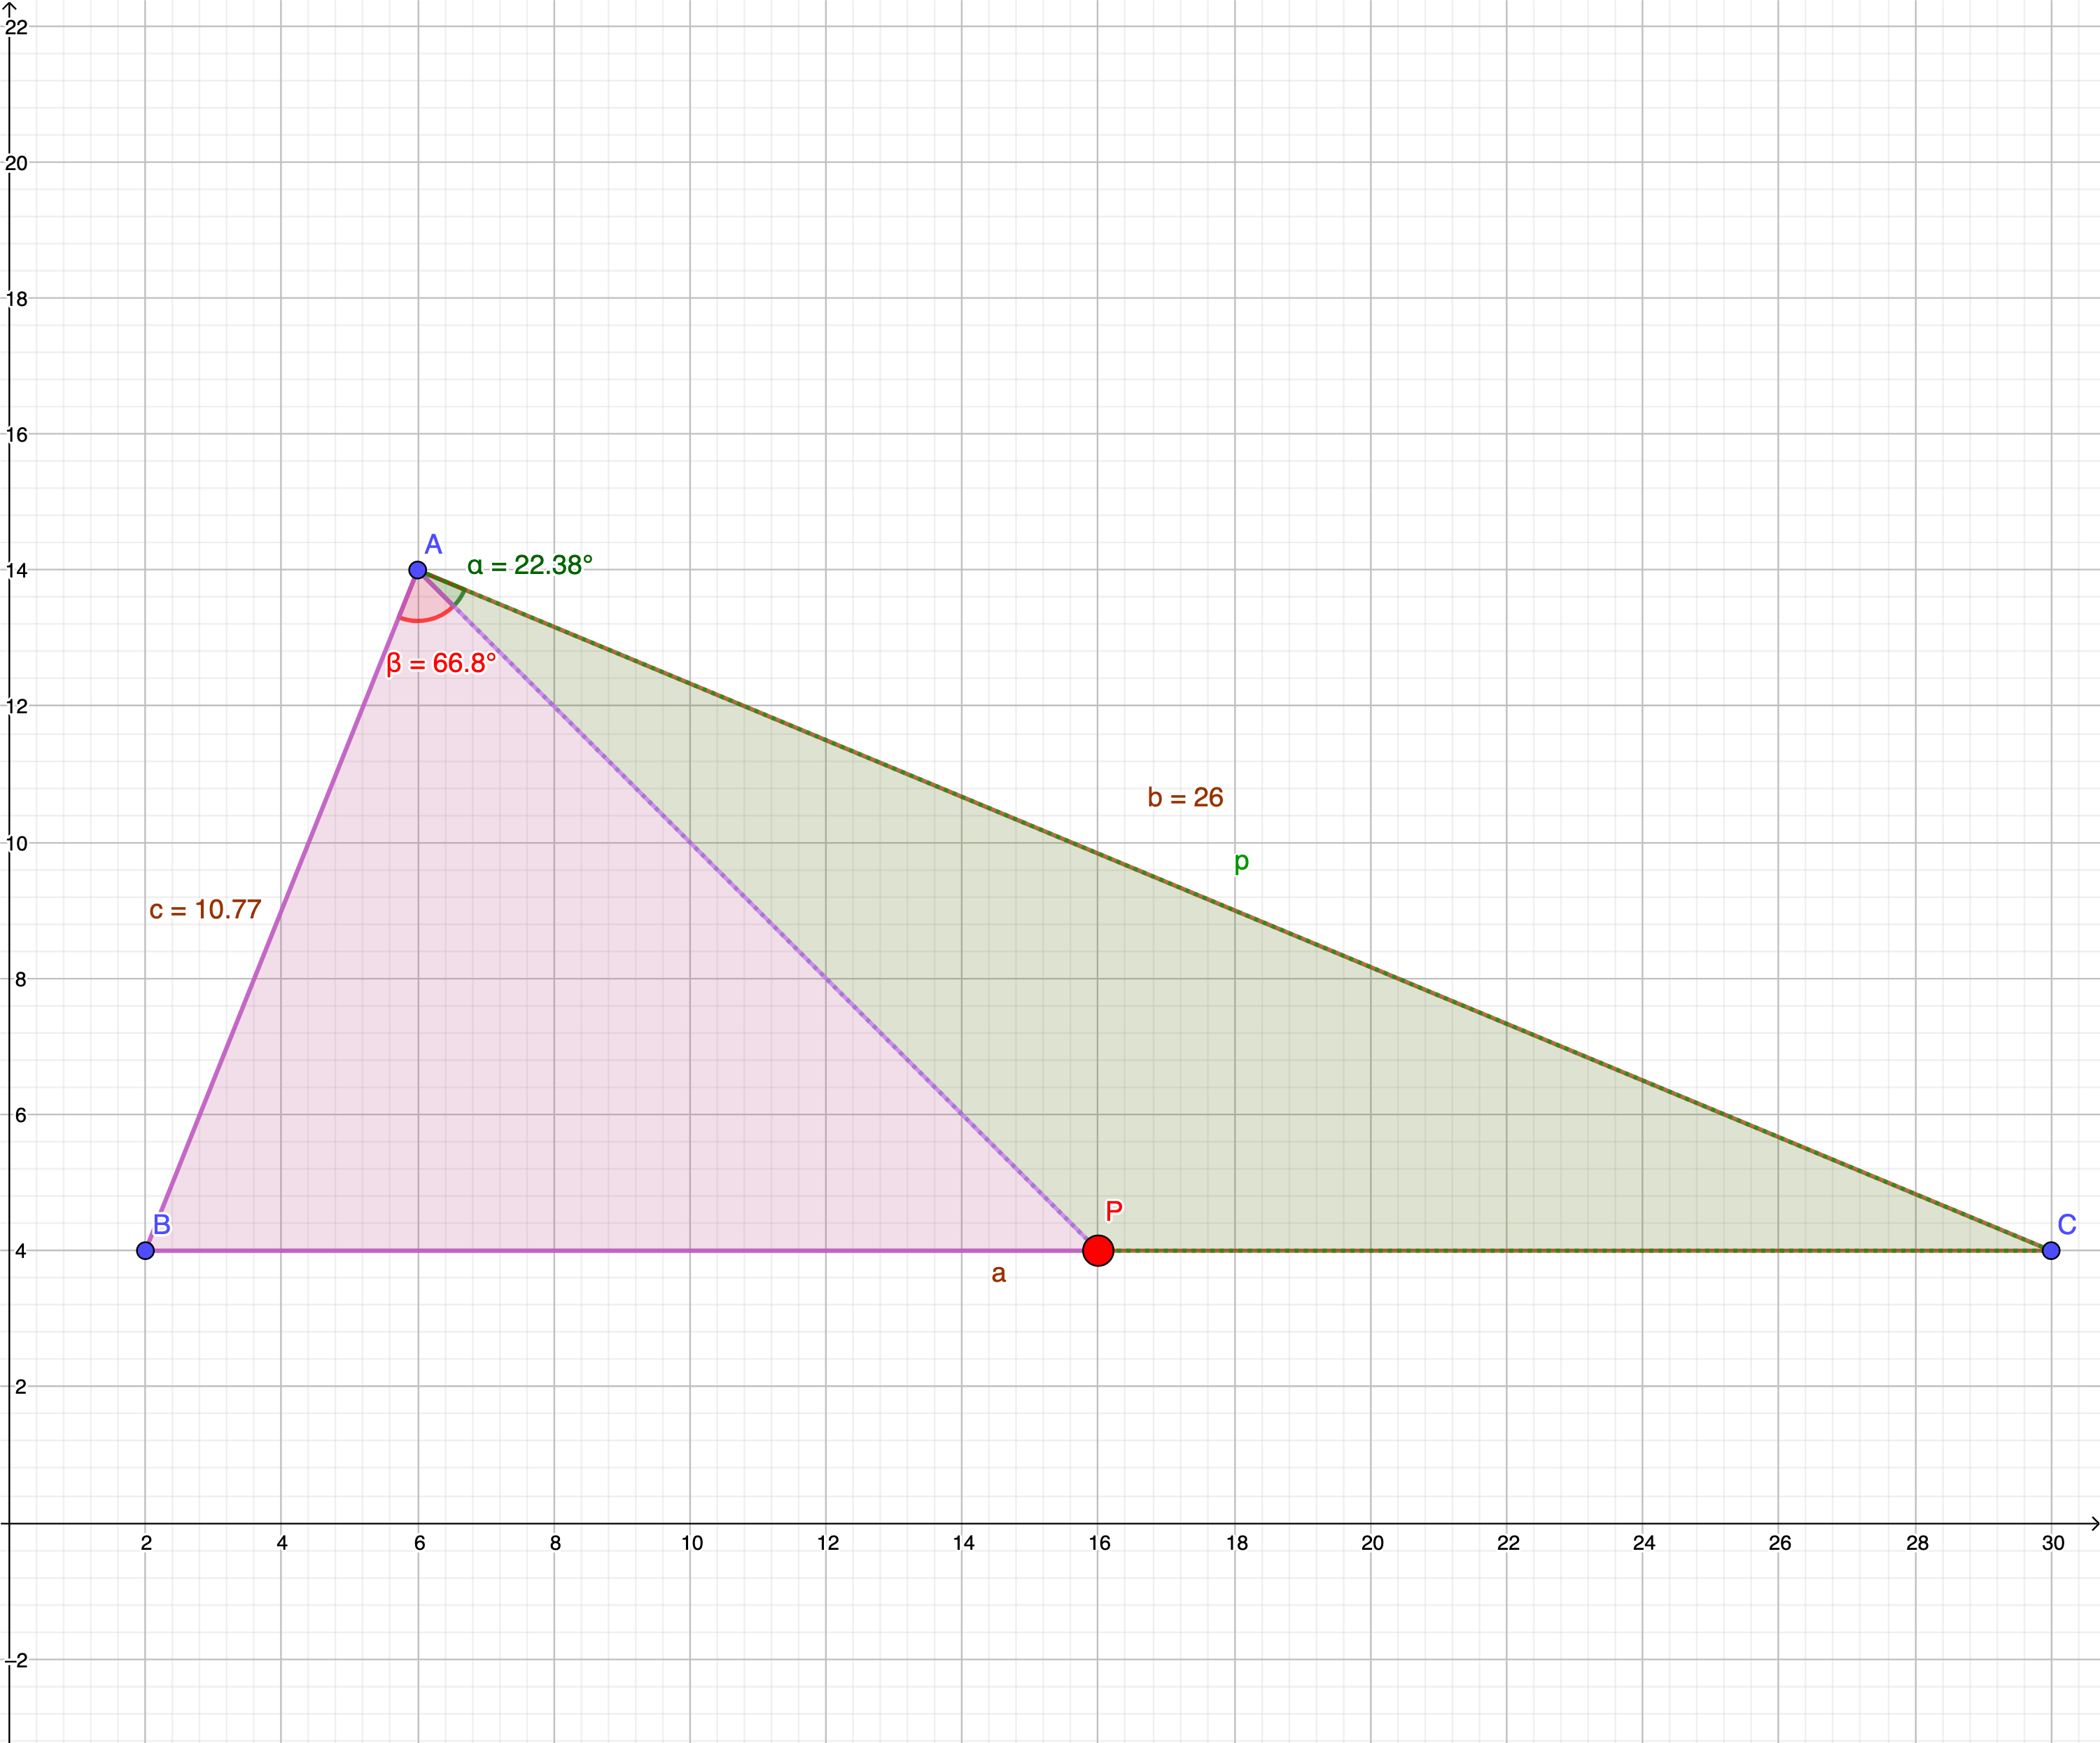
\includegraphics[scale=0.5]{Images/P5.png}
	\caption{Construcción}
\end{figure}

\begin{proof}
	Dado un $\triangle ABC$. A probar: $\angle PAC< \angle BAP$. Por hipótesis tenemos: $P=\frac{1}{2}(B+C)$, que también se podría expresar como $BP=PC$ y $AB<AC$. Ahora bien, notamos que la condición se cumple trivialmente por el teorema de la bisectriz generalizado tal que, 
	$$\frac{BP}{PC}=\frac{AB\sen BAP}{CA\sen PAC}\implies \frac{CA}{AB}=\frac{\sen BAP}{\sen PAC}.$$
	
	$\therefore \ $ Por proporcionalidad, $\angle PAC< \angle BAP$.
	
\end{proof}
















%---------------------------
\bibliographystyle{apa}
\bibliography{referencias.bib}

\end{document}